\documentclass[11pt,aspectratio=43,usenames,dvipsnames]{beamer}
\usepackage[utf8]{inputenc}
\usepackage{amsmath, amsfonts, amssymb, amsthm}
\usepackage[T1]{fontenc}
% mint: code chuck and syntax highlighting
%% outputdir should change according to pdf build directory
% \usepackage[outputdir=build,cache=false]{minted}
\usepackage{lmodern}
\usepackage{xcolor}
\usepackage{setspace}
\usepackage{booktabs}
\usepackage{multirow}
\usepackage{graphicx}
\usepackage{tikz}
% \usetikzlibrary{decorations}
\usetikzlibrary{decorations.pathreplacing, intersections}
\usepackage{ulem}
\usepackage{hyperref}
\usepackage{booktabs}
\usepackage{babel}
\usepackage{makecell}
\usepackage[para,online,flushleft]{threeparttable}
\usepackage{pdfpages}
\usepackage{tcolorbox}
\usepackage{bm}
\usepackage{appendixnumberbeamer}
\usepackage{natbib}
\usepackage{caption}
\captionsetup[figure]{labelformat=empty}% redefines the caption setup of the figures environment in the beamer class.
\usetheme[compress]{Boadilla}
\usecolortheme{default}
\useoutertheme{miniframes}
\usefonttheme[onlymath]{serif}

\newcommand{\jump}[2]{\hyperlink{#1}{\beamerbutton{#2}}}
\newcommand{\orange}[1]{\textcolor{orange}{#1}}
\newcommand{\red}[1]{\textcolor{red}{#1}}
\newcommand{\blue}[1]{\textcolor{blue}{#1}}
\newcommand{\green}[1]{\textcolor{OliveGreen}{#1}}

\renewcommand{\square}{\scalebox{0.7}{$\blacksquare$ \hspace{0.5em}}}
\setbeamertemplate{itemize item}{\raisebox{0.1em}{\scalebox{0.7}{$\blacksquare$}}}
\setbeamertemplate{itemize subitem}[circle]
\setbeamertemplate{itemize subsubitem}{--}
\setbeamercolor{itemize item}{fg=black}
\setbeamercolor{itemize subitem}{fg=black}
\setbeamercolor{itemize subsubitem}{fg=black}
\setbeamercolor{item projected}{bg=darkgray,fg=white}
\definecolor{blue}{rgb}{0.2, 0.2, 0.7}
\setbeamercolor{alerted text}{fg=blue}
\setbeamertemplate{enumerate items}[circle]


\setbeamertemplate{headline}{}

%==========================================
\let\olditemize=\itemize
\let\endolditemize=\enditemize
\renewenvironment{itemize}{\olditemize \itemsep1em}{\endolditemize}
\let\oldenumerate=\enumerate
\let\endoldenumerate=\endenumerate
\renewenvironment{enumerate}{\oldenumerate \itemsep1em}{ \endoldenumerate}

\DeclareMathOperator*{\argmax}{\arg\!\max}
\DeclareMathOperator*{\E}{\mathbb{E}}
\DeclareMathOperator*{\var}{\rm Var}
\DeclareMathOperator*{\cov}{\rm Cov}

\theoremstyle{definition}
\newtheorem{assume}{Assumption}
\newtheorem{lem}{Lemma}
\newtheorem{proposition}{Proposition}
\newtheorem{thm}{Theorem}
\newtheorem{corol}{Corollary}

\AtBeginSection[]{
  \begin{frame}[noframenumbering]
  \vfill
  \centering
  \begin{beamercolorbox}[sep=8pt,center,shadow=true,rounded=true]{title}
    \usebeamerfont{title}\insertsection\par%
  \end{beamercolorbox}
  \vfill
  \end{frame}
}

% \BeforeBeginEnvironment{frame}{%
%  \setbeamertemplate{footline}[split theme]
% }

% \makeatletter
% \define@key{beamerframe}{standout}[true]{%
% \setbeamertemplate{footline}{}%
% }
% \makeatother

\begin{document}
    \title[Unit 1]{Unit 1 \\ The Capitalist Revolution}
    \author[Hui-Jun Chen]{Hui-Jun Chen}
    \institute[OSU]{The Ohio State University}
    % \date{\today}
    \date{\today}
    \setbeamertemplate{navigation symbols}{}
    \setstretch{1.2}

%-------------------------------------------------------
{
%	\usebackgroundtemplate{\includegraphics[width=1\paperwidth]{../EveningSky_cropped_edit43_bright.jpg}}
    \begin{frame}
% \vspace{3em}
        \centering
%		{\footnotesize 	ECON 4002 Intermediate Macroeconomic Theory}
        \maketitle
% \vspace{-1.5em}
% \centering
% \includegraphics[width=0.55\linewidth]{Pictures/houses.jpeg}


    \end{frame}
}

% -------------------------------------------
\setbeamertemplate{headline}
{
\setbeamercolor{section in head/foot}{fg=black, bg=white}
\vskip1em \tiny \insertsectionnavigationhorizontal{1\paperwidth}{\hspace{0.50\paperwidth}}{}
}
%------------------------------------------

\section[Intro]{Introduction}
\label{sec:Introduction}

\begin{frame}{Flat v.s. Spiky World}
\label{slide:Flat_v_s__Spiky_World}
    \begin{center}
        Is Capitalism Good or Bad to this world?
    \end{center}

    \begin{itemize}
        \item Flat v.s. Spiky: equal v.s. unequal wealth/income distribution
        \item Before industrial revolution: flat world but lower living standard
        \item After industrial revolution: spiky world but higher living standard
        \item Interactive figure: \blue{\url{https://tinyco.re/3290463}}
        \begin{itemize}
            \item Rapid, sustained growth starts at industrial revolution
            \item Growth starts as the country started the industrialization
        \end{itemize}
        \item Key factor of industrial revolution: \blue{capital \& capitalist}
        \item If you want read more: \blue{\url{https://tinyurl.com/2ud7vc8z}}
    \end{itemize}

\end{frame}

\section{Inequality}
\label{sec:Inequality}

\begin{frame}{How do we measuring income \& living standard?}
\label{slide:How_do_we_measuring_income____living_standard_}
    \begin{enumerate}
        \item \textbf{GDP per capita}: GDP per person.
        \begin{itemize}
            \item \textbf{GDP} (Gross domestic product): market value of \blue{final goods} and \blue{services} \textit{within countries} in a year.
            \item GDP per capita $ = \frac{\text{GDP}}{\text{population}} $
        \end{itemize}
        \item \textbf{Disposable income}: Income $ -  $ taxes $ + $ gov transfer
    \end{enumerate}

    \vspace{1em}

    \begin{itemize}
        \item Are they precise measure of ``\textbf{well-being}''? Probably not!
        \item Not all aspects of well-being can be captured by these numbers, and
        \item Not all aspects of the world can/should be explained by Economics!
        \item But these numbers indeed allow us to compare wealth/income change across countries and time.
    \end{itemize}

\end{frame}

\begin{frame}{Spikiness: evolution of inequality}
\label{slide:Spikiness__evolution_of_inequality}
    \begin{itemize}
        \item Interactive figure: \blue{\url{https://tinyco.re/7434364}}
        \item Within-country: the rich owns much more then the poor
        \item Between-country: wealth gap between top 10\% and buttom 10\% countries are wider
        \begin{enumerate}
            \item The richest 10\% and poorest 10\%
            \begin{itemize}
                \item Singapore: \$67,436 and \$3,652 v.s. Liberia: \$994 and \$17
            \end{itemize}
            \item Income distribution shifts:
            \begin{itemize}
                \item 1980: poorest $ \Rightarrow  $ Lesotho \& China; richest $ \Rightarrow  $ Switzerland, Finland, US
                \item 1990: China $ \uparrow  $
                \item 2014: China $ \uparrow \uparrow  $; developed countries still top
            \end{itemize}
        \end{enumerate}
    \end{itemize}
\end{frame}

\section[Growth]{``Hockey-stick'' Growth}
\label{sec:__Hockey_stick___Growth}

\begin{frame}{Growth in income}
\label{slide:Growth_in_income}
    \begin{itemize}
        \item growth rate $ = \frac{\text{change in income}}{\text{original level of income}}$
        \item Interactive figure: \blue{\url{https://tinyco.re/3125412}}
        \item Before 1800 we have fewer data points
        \item Country-wise difference:
        \begin{enumerate}
            \item Britain: The hockey-stick kink is less abrupt, began around 1650.
            \item Japan: In Japan the kink is more defined, occurring around 1870.
            \item China and India: The kink happened in the second half of 20th century. GDP per capita actually fell in India during British colonial rule.
        \end{enumerate}
        \item Log/ratio scale $ \Rightarrow  $ recent growth rate in China and Japan > elsewhere
    \end{itemize}
\end{frame}

\begin{frame}{Technological \& Industrial Revolution}
\label{slide:Technological____Industrial_Revolution}
    \begin{center}
        Why the timing and rate of growth are different?
    \end{center}
    \begin{itemize}
        \item \textbf{Technology}: Inputs $ \underbrace{\Longrightarrow}_{\text{Technology}}  $ Output
        \item Industrial Revolution: efficiency in technology $ \uparrow \uparrow  $
        \begin{itemize}
            \item Started at Britain in the 18th century
            \item Example: lighting efficiency is hugely greater than ancestors
            \begin{itemize}
                \item Campfire v.s. Fluorescent bulbs: 45000 times more efficient
            \end{itemize}
        \end{itemize}
        \item The speed of information $ \uparrow \uparrow  $, created a connected world
        \begin{itemize}
            \item 1000-1780: 1 MPH (Horse, bird) $ \rightarrow  $ 1865: 12 MPH (Telegraphy)
        \end{itemize}
    \end{itemize}
\end{frame}

\begin{frame}{Environmental Consequences}
\label{slide:Environmental_Consequences}
    \begin{itemize}
        \item Interactive figure: \blue{\url{https://tinyco.re/8926412}}
        \item Increase production \& population had impact on the environment:
        \begin{itemize}
            \item Global: climate change \& extreme weather phenomenon
            \item Local: pollution in the city \& deforestation
        \end{itemize}
        \item The impacts are the result of
        \begin{itemize}
            \item expansion of the economy: growth in total output
            \item how economy is organized: what is valued to human?
        \end{itemize}
        \item Technology as the cause may also be the solution (at least I hope)
        \item But, even not the solution, shouldn't be the reason for \blue{demoralization}
    \end{itemize}


\end{frame}

\section{Capitalism}
\label{sec:Capitalism}

\begin{frame}{Definition of Capitalism}
\label{slide:Definition_of_Capitalism}
    \begin{itemize}
        \item Capitalism is an \alert{economic system} constituted by
        \begin{enumerate}
            \item a society that protects private property (e.g. Fifth Amendment),
            \item markets with medium of exchange that all agreed upon (e.g. US\$),
            \item firms that owns capital, hiring labor and produce goods for profit
        \end{enumerate}
    \end{itemize}

    \begin{center}
        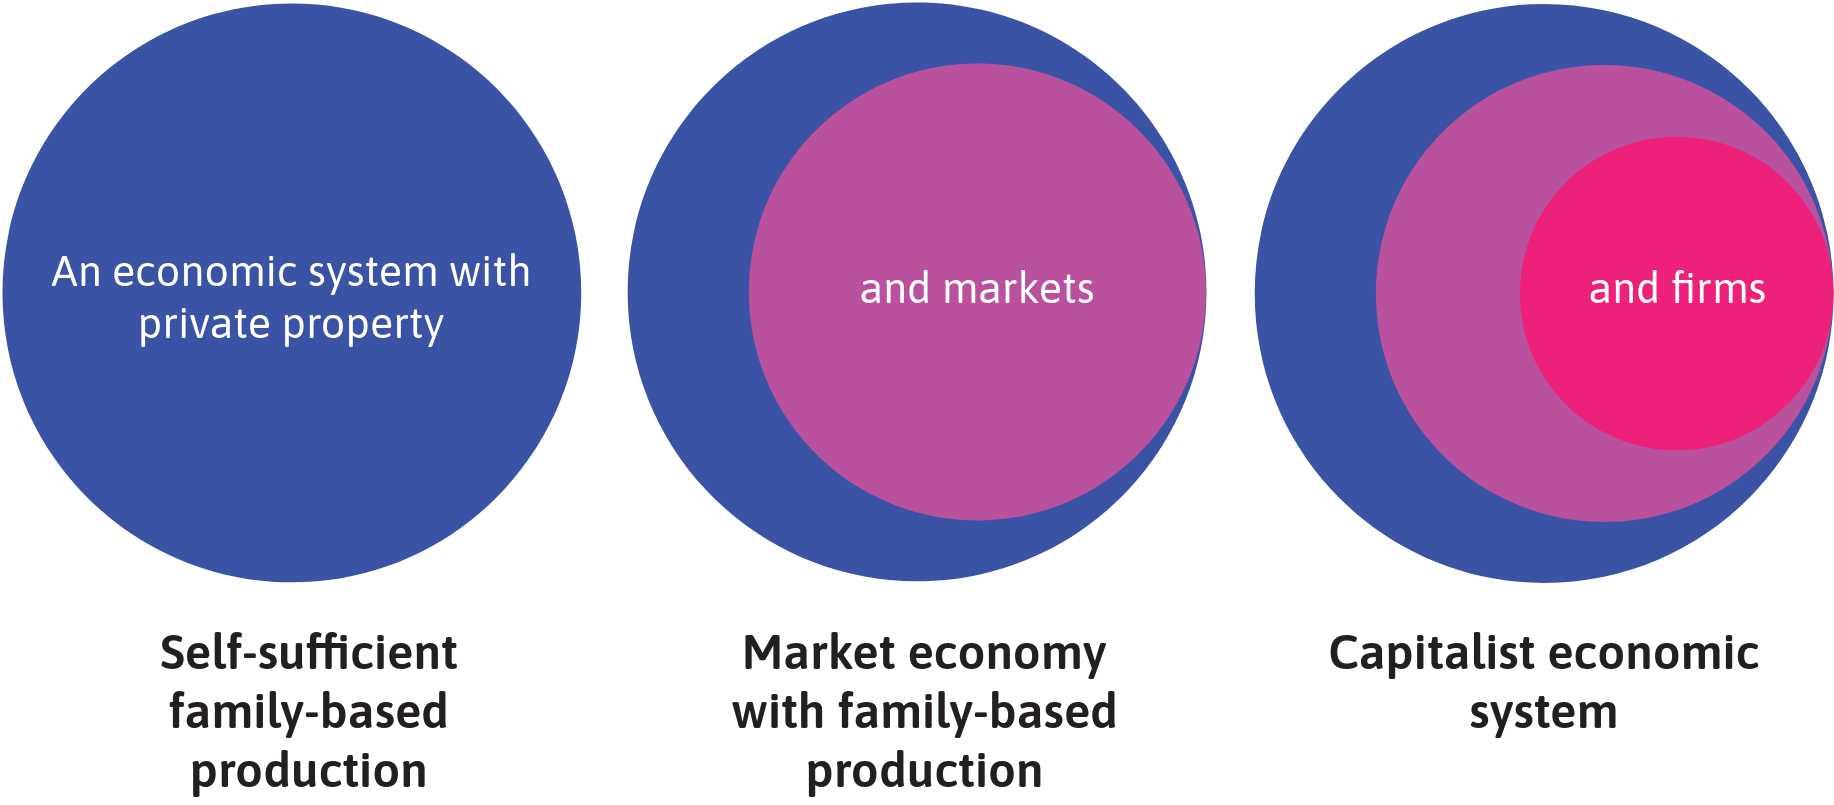
\includegraphics[width=0.9\textwidth]{./figures/Figure1_8.png}
    \end{center}

\end{frame}

\begin{frame}{Components of Capitalism}
\label{slide:Components_of_Capitalism}
    \begin{enumerate}
        \item Private property: \blue{legislative} guarantee to exclude others from use/exchange
        \item Capital: durable non-labor inputs used in production
        \begin{itemize}
            \item e.g. machine, building
            \item air \& water are mostly $ 0 $ cost in production $ \Rightarrow  $ slide \ref{slide:Environmental_Consequences}
        \end{itemize}
        \item Markets: where trade voluntarily happened for self benefit
        \item Firms: private \textbf{owners of capital} hire \textbf{labor} to produce goods and services to \textbf{trade in the markets} in pursue of \textbf{profit}
        \begin{itemize}
            \item Family or individual production \textit{not hiring}
            \item Nonprofit organization \textit{not pursuing profit}
            \item Government bodies \textit{not pursing profit and not own capital}
        \end{itemize}

    \end{enumerate}


\end{frame}

\begin{frame}{The Capitalist Revolution}
\label{slide:The_Capitalist_Revolution}
    Capitalism \& Industrial Revolution increases living standard because
    \begin{enumerate}
        \item \textbf{Competition}: the desire to pursue profit leads to better technologies
        \item \textbf{Specialization}: markets allow institution to develop \alert{comparative advantage} in production
        \item \textbf{Comparative advantage}: how much \alert{sacrifice} I need to make in order to produce \alert{1 good}? (sacrifice: opportunity cost)
    \end{enumerate}
    \begin{tabular}{cc}
        if put 100\% time in one good
        \\
        \begin{tabular}{ccc}
                & apples
                & wheat
            \\
            John
                & 1250
                & 50
            \\
            David
                & 1000
                & 20
            \\
        \end{tabular}
    \end{tabular}
    $ \Longrightarrow $
    \begin{tabular}{cc}
        sacrifice made to produce 1 good
        \\
        \begin{tabular}{ccc}
                & apples
                & wheat
            \\
            John
                & 0.04 wheat
                & 25 apple
            \\
            David
                & 0.02 wheat
                & 50 apple
            \\
        \end{tabular}
    \end{tabular}

    John has \textbf{absolute advantage} in both goods, but David has \textbf{comparative advantage} in wheat!
\end{frame}

\begin{frame}{Did capitalism \textit{cause} the hockey-stick growth?}
\label{slide:Did_capitalism__textit_cause__the_hockey_stick_growth_}
\textit{Natural experiment}: Division of West and East Germany and the end of WWII shows the power of capitalism \href{https://tinyco.re/19372660}{\beamergotobutton{Figure}}

    \begin{center}
        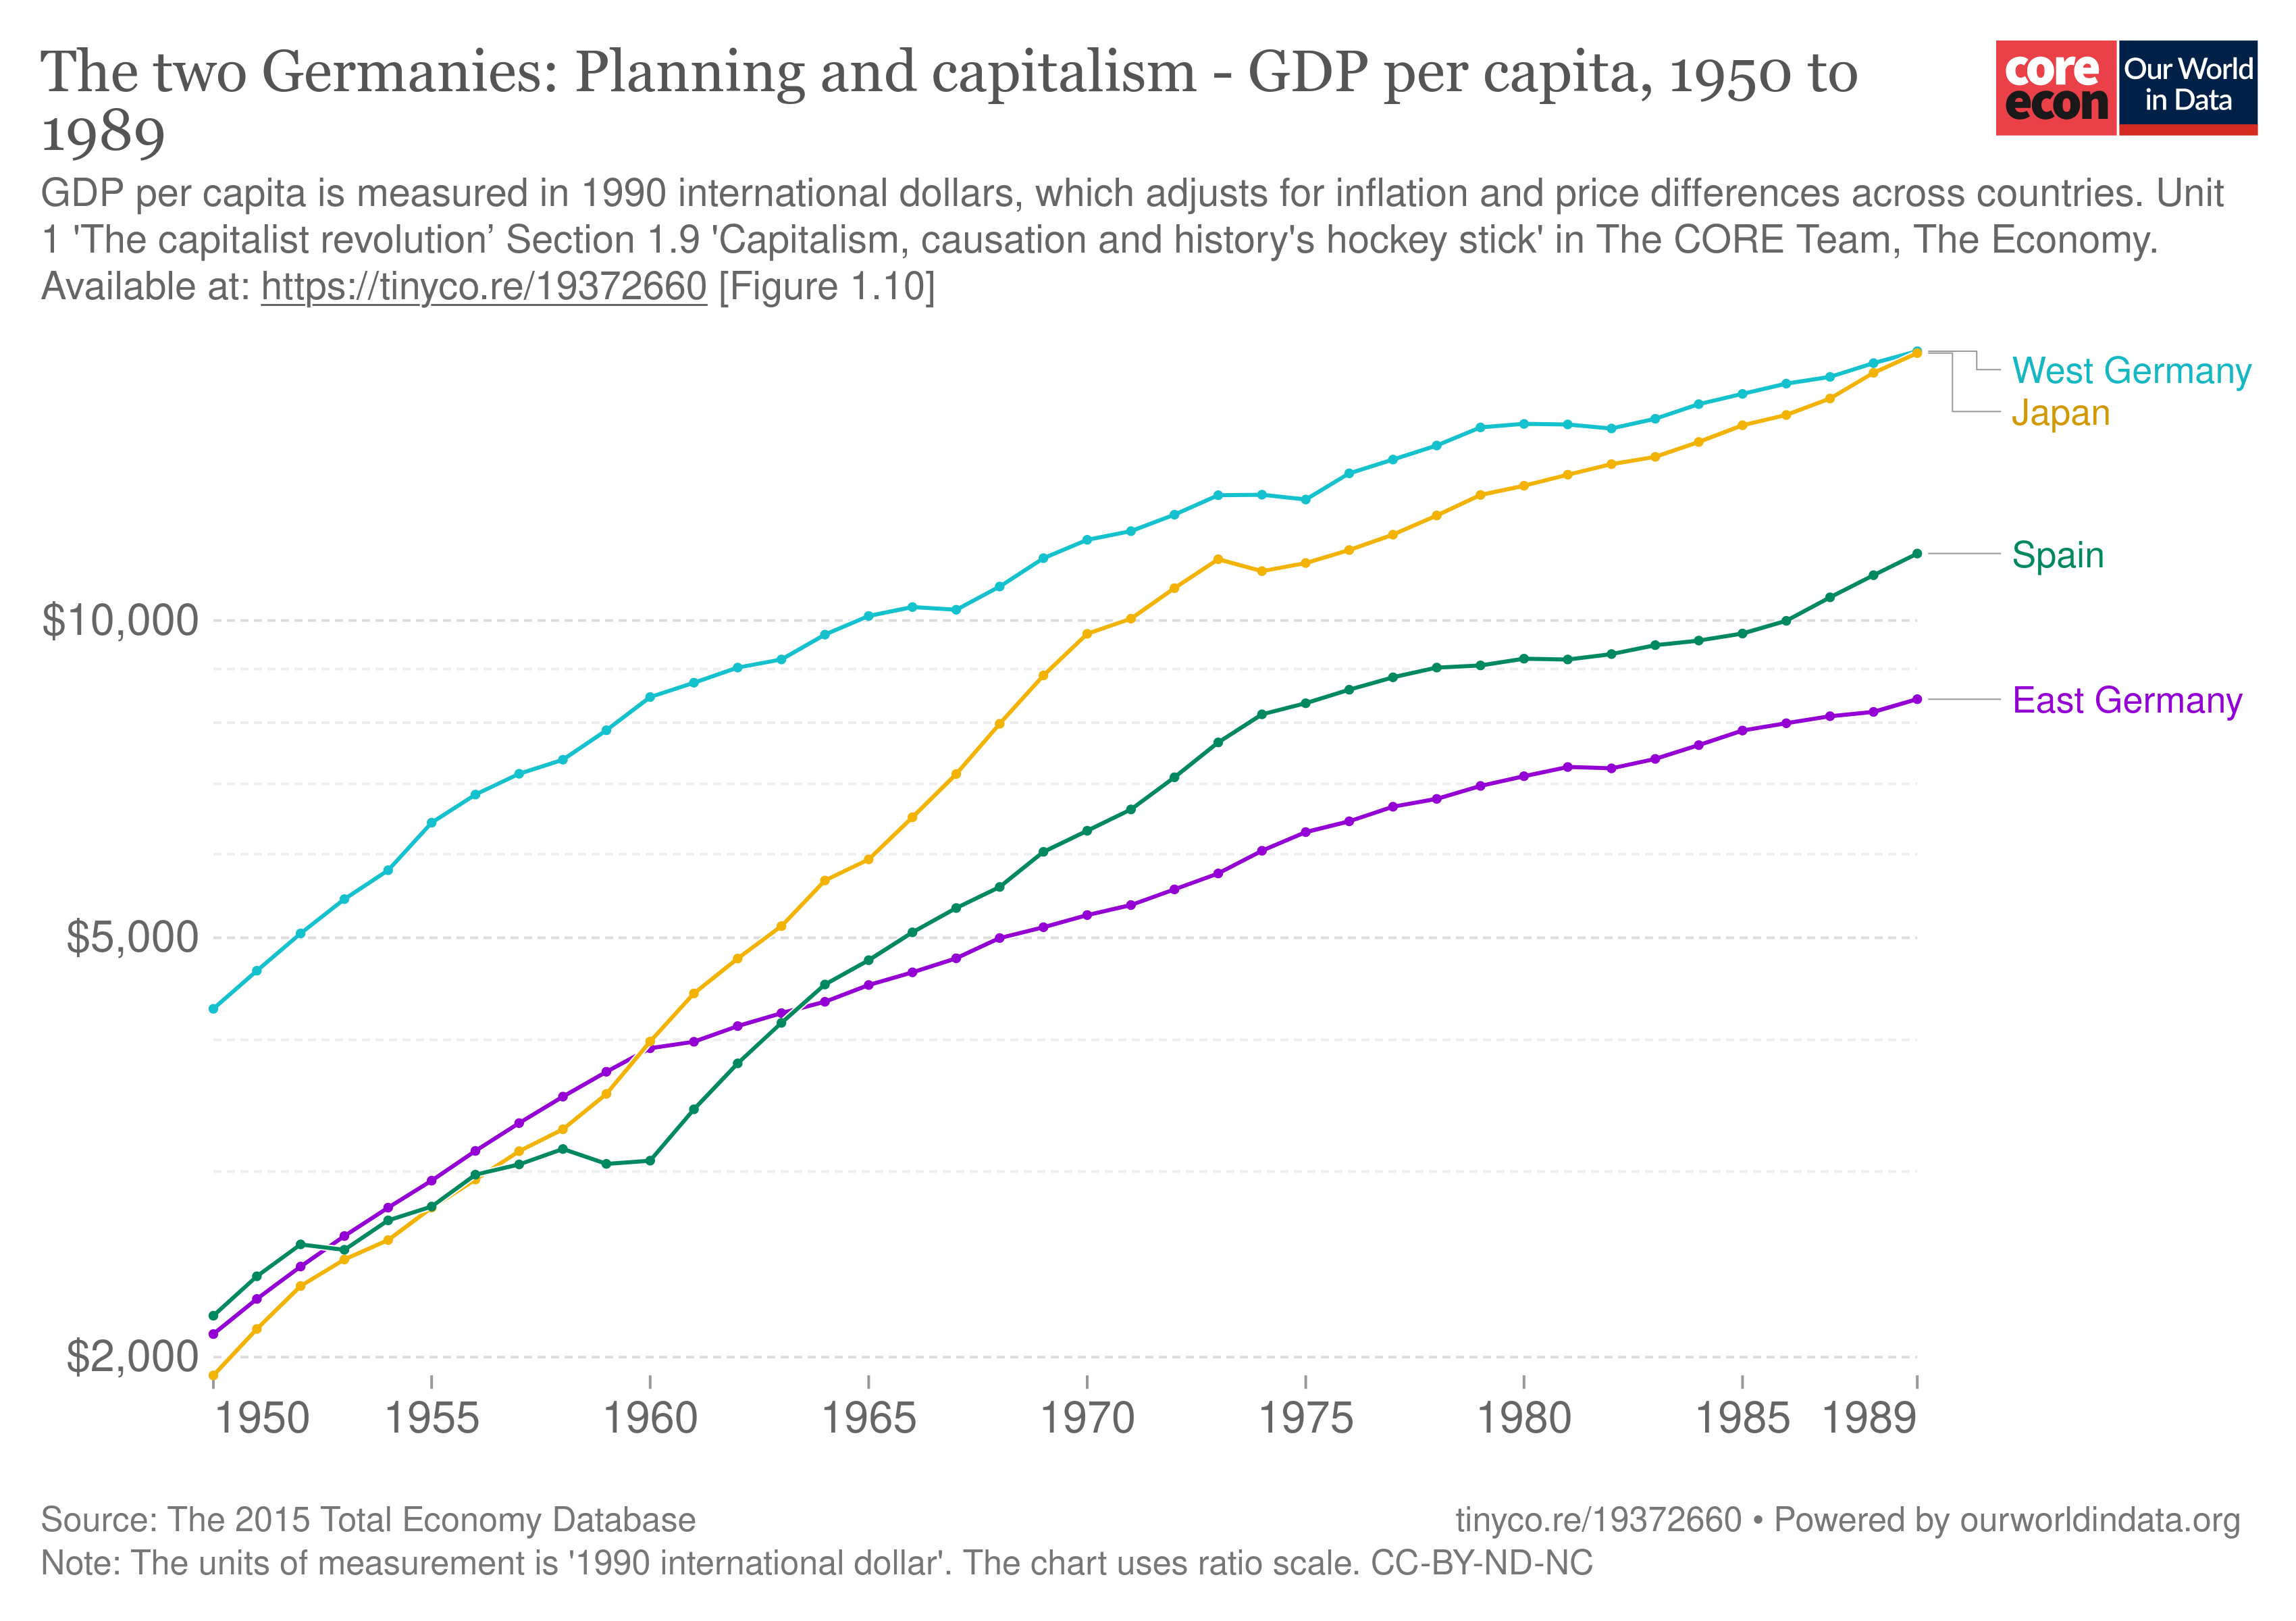
\includegraphics[width=0.8\textwidth]{./figures/the-two-germanies-planning-and-capitalism.png}
    \end{center}
\end{frame}

\begin{frame}{Success are not equal}
\label{slide:Success_are_not_equal}
    All \textbf{economics conditions}, \textbf{political stability}, and \textbf{government functionality} matters

    Capitalism coexists with \textit{democracy} in most countries
    \begin{center}
        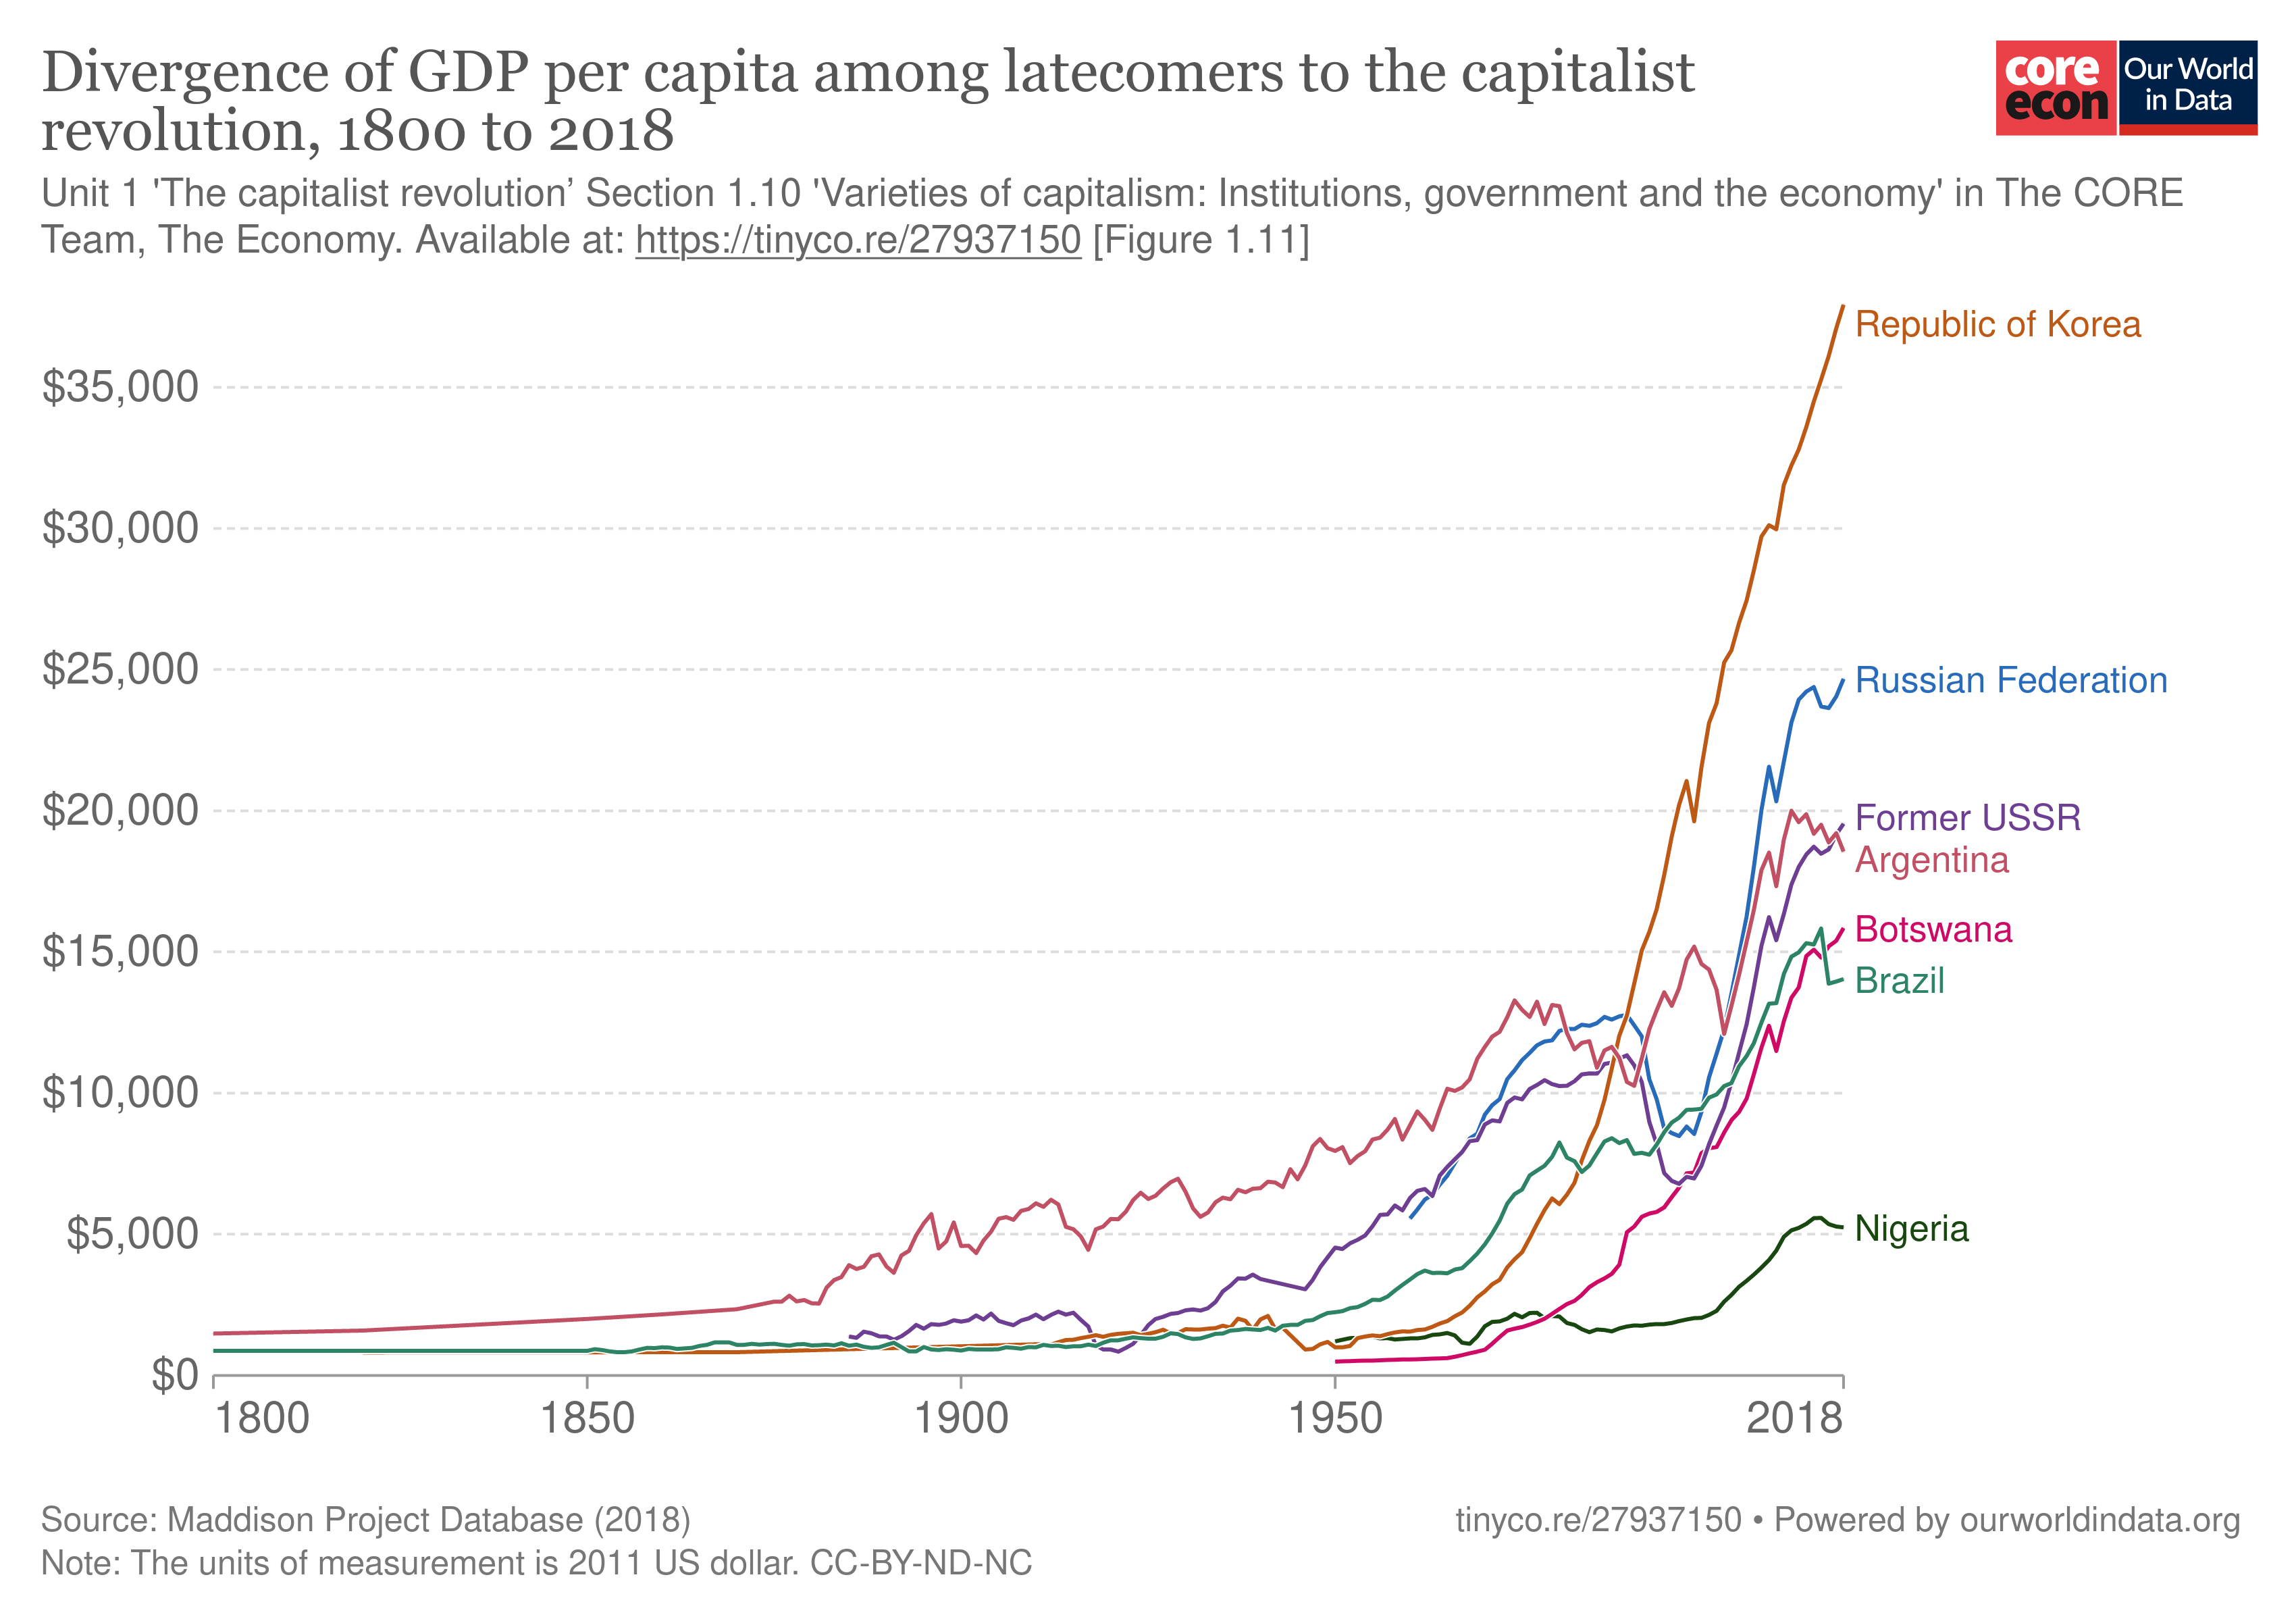
\includegraphics[width=0.75\textwidth]{./figures/divergence-of-gdp-per-capita-among-latecomers-to-the-capitalist-revolution-18002016.png}
    \end{center}
\end{frame}

\section{Economics}
\label{sec:Economics}

\begin{frame}{What is Economics?}
\label{slide:What_is_Economics_}
    \begin{center}
        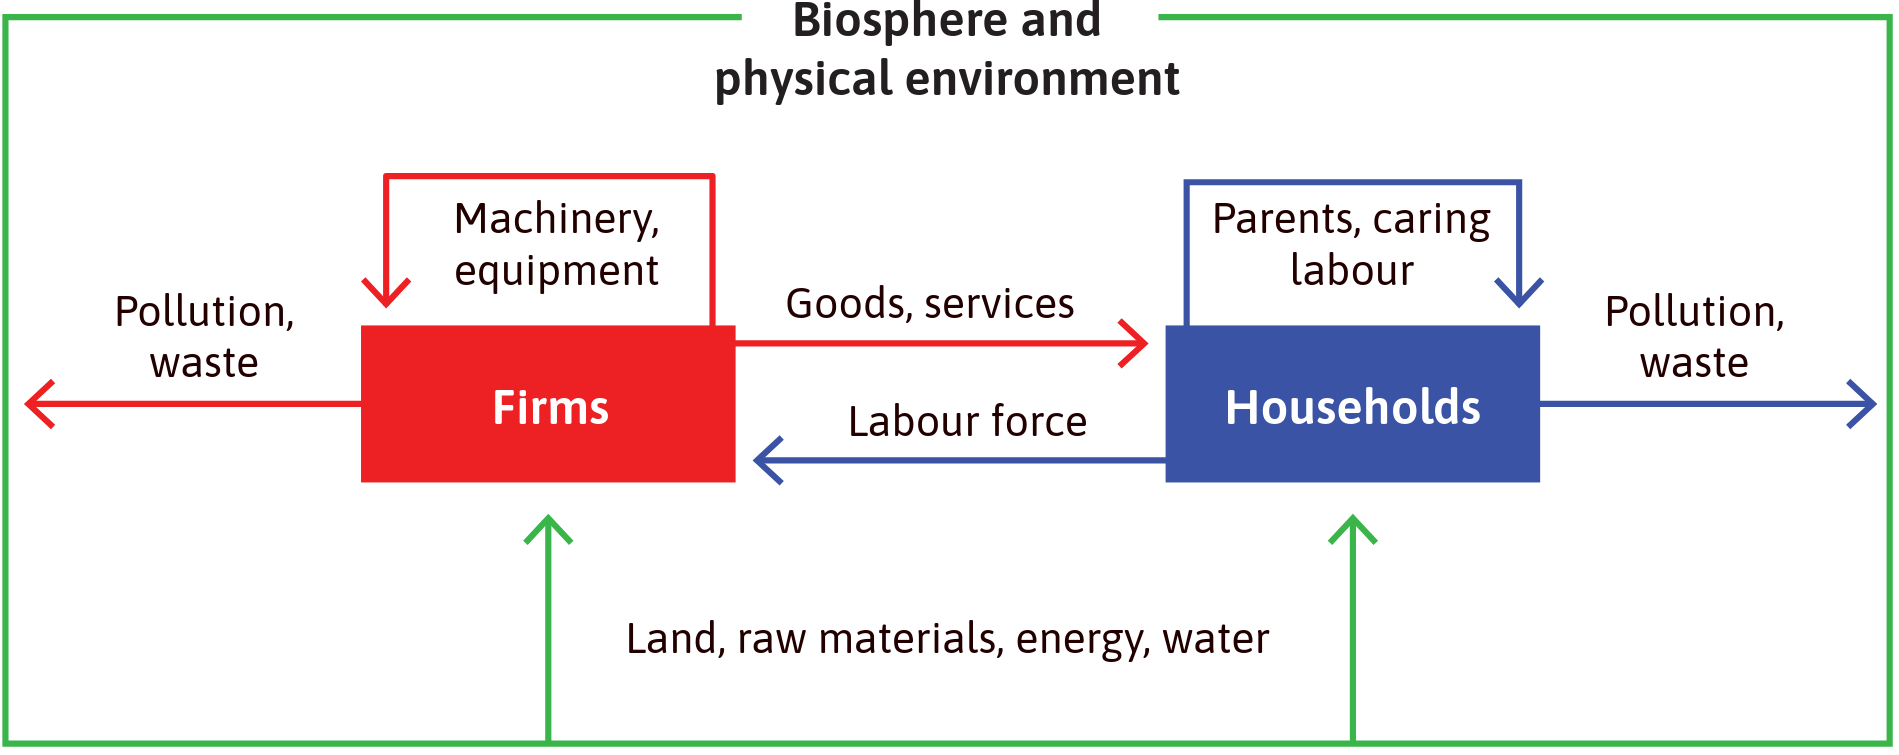
\includegraphics[width=0.9\textwidth]{./figures/Figure1_15.png}
    \end{center}
    Economics is a \alert{scientific pursuit} involving the formulation and \alert{refinement of theories} that can help us better understand \alert{how economies work} and \alert{how they can be improved}
\end{frame}

\end{document}
